\documentclass[crop,tikz,convert={outext=.svg,command=\unexpanded{pdf2svg \infile\space\outfile}},multi=false]{standalone}[2012/04/13]
%\usetikzlibrary{...}% tikz package already loaded by 'tikz' option
\makeatletter
\begin{document}
	% Created by tikzDevice version 0.12.3 on 2019-09-06 09:57:29
	% !TEX encoding = UTF-8 Unicode
	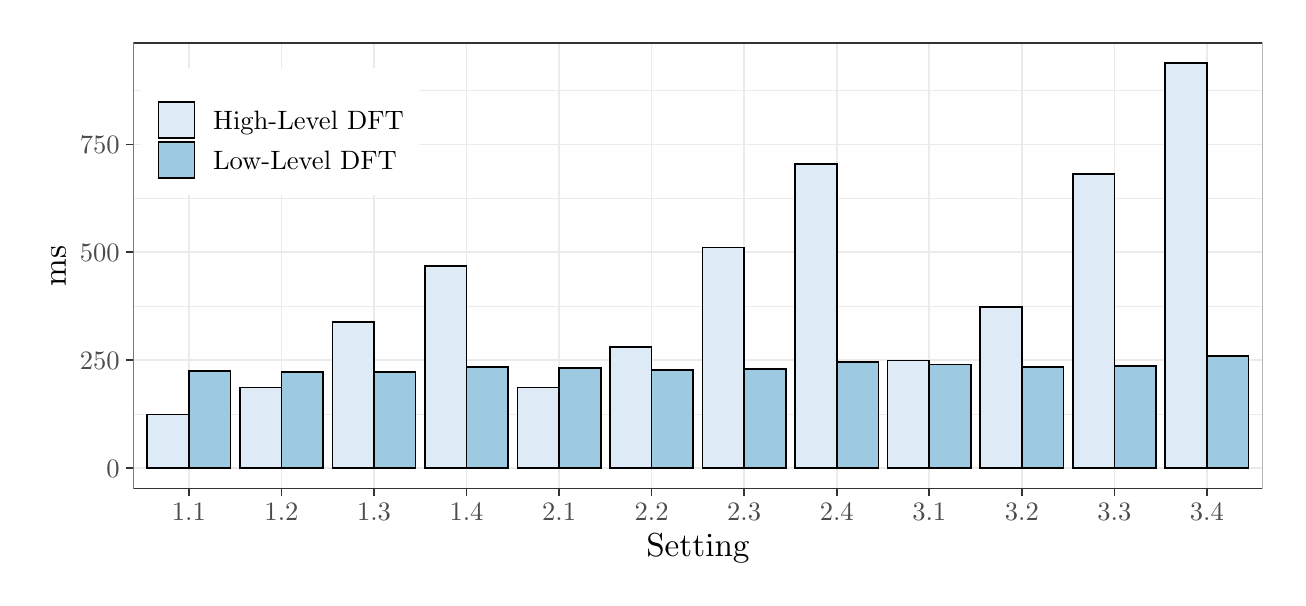
\begin{tikzpicture}[x=1pt,y=1pt]
	\definecolor{fillColor}{RGB}{255,255,255}
	\path[use as bounding box,fill=fillColor,fill opacity=0.00] (0,0) rectangle (451.69,198.74);
	\begin{scope}
	\path[clip] (  0.00,  0.00) rectangle (451.69,198.74);
	\definecolor{drawColor}{RGB}{255,255,255}
	\definecolor{fillColor}{RGB}{255,255,255}
	
	\path[draw=drawColor,line width= 0.6pt,line join=round,line cap=round,fill=fillColor] (  0.00,  0.00) rectangle (451.69,198.74);
	\end{scope}
	\begin{scope}
	\path[clip] ( 38.19, 32.28) rectangle (446.19,193.24);
	\definecolor{fillColor}{RGB}{255,255,255}
	
	\path[fill=fillColor] ( 38.19, 32.28) rectangle (446.19,193.24);
	\definecolor{drawColor}{gray}{0.92}
	
	\path[draw=drawColor,line width= 0.3pt,line join=round] ( 38.19, 59.09) --
	(446.19, 59.09);
	
	\path[draw=drawColor,line width= 0.3pt,line join=round] ( 38.19, 98.09) --
	(446.19, 98.09);
	
	\path[draw=drawColor,line width= 0.3pt,line join=round] ( 38.19,137.09) --
	(446.19,137.09);
	
	\path[draw=drawColor,line width= 0.3pt,line join=round] ( 38.19,176.08) --
	(446.19,176.08);
	
	\path[draw=drawColor,line width= 0.6pt,line join=round] ( 38.19, 39.59) --
	(446.19, 39.59);
	
	\path[draw=drawColor,line width= 0.6pt,line join=round] ( 38.19, 78.59) --
	(446.19, 78.59);
	
	\path[draw=drawColor,line width= 0.6pt,line join=round] ( 38.19,117.59) --
	(446.19,117.59);
	
	\path[draw=drawColor,line width= 0.6pt,line join=round] ( 38.19,156.58) --
	(446.19,156.58);
	
	\path[draw=drawColor,line width= 0.6pt,line join=round] ( 58.26, 32.28) --
	( 58.26,193.24);
	
	\path[draw=drawColor,line width= 0.6pt,line join=round] ( 91.70, 32.28) --
	( 91.70,193.24);
	
	\path[draw=drawColor,line width= 0.6pt,line join=round] (125.14, 32.28) --
	(125.14,193.24);
	
	\path[draw=drawColor,line width= 0.6pt,line join=round] (158.59, 32.28) --
	(158.59,193.24);
	
	\path[draw=drawColor,line width= 0.6pt,line join=round] (192.03, 32.28) --
	(192.03,193.24);
	
	\path[draw=drawColor,line width= 0.6pt,line join=round] (225.47, 32.28) --
	(225.47,193.24);
	
	\path[draw=drawColor,line width= 0.6pt,line join=round] (258.91, 32.28) --
	(258.91,193.24);
	
	\path[draw=drawColor,line width= 0.6pt,line join=round] (292.35, 32.28) --
	(292.35,193.24);
	
	\path[draw=drawColor,line width= 0.6pt,line join=round] (325.80, 32.28) --
	(325.80,193.24);
	
	\path[draw=drawColor,line width= 0.6pt,line join=round] (359.24, 32.28) --
	(359.24,193.24);
	
	\path[draw=drawColor,line width= 0.6pt,line join=round] (392.68, 32.28) --
	(392.68,193.24);
	
	\path[draw=drawColor,line width= 0.6pt,line join=round] (426.12, 32.28) --
	(426.12,193.24);
	\definecolor{drawColor}{RGB}{0,0,0}
	\definecolor{fillColor}{RGB}{158,202,225}
	
	\path[draw=drawColor,line width= 0.6pt,line cap=rect,fill=fillColor] ( 58.26, 39.59) rectangle ( 73.31, 74.58);
	\definecolor{fillColor}{RGB}{222,235,247}
	
	\path[draw=drawColor,line width= 0.6pt,line cap=rect,fill=fillColor] ( 43.21, 39.59) rectangle ( 58.26, 58.99);
	\definecolor{fillColor}{RGB}{158,202,225}
	
	\path[draw=drawColor,line width= 0.6pt,line cap=rect,fill=fillColor] ( 91.70, 39.59) rectangle (106.75, 74.21);
	\definecolor{fillColor}{RGB}{222,235,247}
	
	\path[draw=drawColor,line width= 0.6pt,line cap=rect,fill=fillColor] ( 76.65, 39.59) rectangle ( 91.70, 68.66);
	\definecolor{fillColor}{RGB}{158,202,225}
	
	\path[draw=drawColor,line width= 0.6pt,line cap=rect,fill=fillColor] (125.14, 39.59) rectangle (140.19, 74.29);
	\definecolor{fillColor}{RGB}{222,235,247}
	
	\path[draw=drawColor,line width= 0.6pt,line cap=rect,fill=fillColor] (110.09, 39.59) rectangle (125.14, 92.37);
	\definecolor{fillColor}{RGB}{158,202,225}
	
	\path[draw=drawColor,line width= 0.6pt,line cap=rect,fill=fillColor] (158.59, 39.59) rectangle (173.63, 76.06);
	\definecolor{fillColor}{RGB}{222,235,247}
	
	\path[draw=drawColor,line width= 0.6pt,line cap=rect,fill=fillColor] (143.54, 39.59) rectangle (158.59,112.62);
	\definecolor{fillColor}{RGB}{158,202,225}
	
	\path[draw=drawColor,line width= 0.6pt,line cap=rect,fill=fillColor] (192.03, 39.59) rectangle (207.08, 75.78);
	\definecolor{fillColor}{RGB}{222,235,247}
	
	\path[draw=drawColor,line width= 0.6pt,line cap=rect,fill=fillColor] (176.98, 39.59) rectangle (192.03, 68.76);
	\definecolor{fillColor}{RGB}{158,202,225}
	
	\path[draw=drawColor,line width= 0.6pt,line cap=rect,fill=fillColor] (225.47, 39.59) rectangle (240.52, 75.06);
	\definecolor{fillColor}{RGB}{222,235,247}
	
	\path[draw=drawColor,line width= 0.6pt,line cap=rect,fill=fillColor] (210.42, 39.59) rectangle (225.47, 83.30);
	\definecolor{fillColor}{RGB}{158,202,225}
	
	\path[draw=drawColor,line width= 0.6pt,line cap=rect,fill=fillColor] (258.91, 39.59) rectangle (273.96, 75.48);
	\definecolor{fillColor}{RGB}{222,235,247}
	
	\path[draw=drawColor,line width= 0.6pt,line cap=rect,fill=fillColor] (243.86, 39.59) rectangle (258.91,119.30);
	\definecolor{fillColor}{RGB}{158,202,225}
	
	\path[draw=drawColor,line width= 0.6pt,line cap=rect,fill=fillColor] (292.35, 39.59) rectangle (307.40, 77.93);
	\definecolor{fillColor}{RGB}{222,235,247}
	
	\path[draw=drawColor,line width= 0.6pt,line cap=rect,fill=fillColor] (277.30, 39.59) rectangle (292.35,149.41);
	\definecolor{fillColor}{RGB}{158,202,225}
	
	\path[draw=drawColor,line width= 0.6pt,line cap=rect,fill=fillColor] (325.80, 39.59) rectangle (340.84, 77.05);
	\definecolor{fillColor}{RGB}{222,235,247}
	
	\path[draw=drawColor,line width= 0.6pt,line cap=rect,fill=fillColor] (310.75, 39.59) rectangle (325.80, 78.44);
	\definecolor{fillColor}{RGB}{158,202,225}
	
	\path[draw=drawColor,line width= 0.6pt,line cap=rect,fill=fillColor] (359.24, 39.59) rectangle (374.29, 76.16);
	\definecolor{fillColor}{RGB}{222,235,247}
	
	\path[draw=drawColor,line width= 0.6pt,line cap=rect,fill=fillColor] (344.19, 39.59) rectangle (359.24, 97.91);
	\definecolor{fillColor}{RGB}{158,202,225}
	
	\path[draw=drawColor,line width= 0.6pt,line cap=rect,fill=fillColor] (392.68, 39.59) rectangle (407.73, 76.58);
	\definecolor{fillColor}{RGB}{222,235,247}
	
	\path[draw=drawColor,line width= 0.6pt,line cap=rect,fill=fillColor] (377.63, 39.59) rectangle (392.68,145.97);
	\definecolor{fillColor}{RGB}{158,202,225}
	
	\path[draw=drawColor,line width= 0.6pt,line cap=rect,fill=fillColor] (426.12, 39.59) rectangle (441.17, 80.01);
	\definecolor{fillColor}{RGB}{222,235,247}
	
	\path[draw=drawColor,line width= 0.6pt,line cap=rect,fill=fillColor] (411.07, 39.59) rectangle (426.12,185.93);
	\definecolor{drawColor}{gray}{0.20}
	
	\path[draw=drawColor,line width= 0.6pt,line join=round,line cap=round] ( 38.19, 32.28) rectangle (446.19,193.24);
	\end{scope}
	\begin{scope}
	\path[clip] (  0.00,  0.00) rectangle (451.69,198.74);
	\definecolor{drawColor}{gray}{0.30}
	
	\node[text=drawColor,anchor=base east,inner sep=0pt, outer sep=0pt, scale=  0.96] at ( 33.24, 36.29) {0};
	
	\node[text=drawColor,anchor=base east,inner sep=0pt, outer sep=0pt, scale=  0.96] at ( 33.24, 75.28) {250};
	
	\node[text=drawColor,anchor=base east,inner sep=0pt, outer sep=0pt, scale=  0.96] at ( 33.24,114.28) {500};
	
	\node[text=drawColor,anchor=base east,inner sep=0pt, outer sep=0pt, scale=  0.96] at ( 33.24,153.28) {750};
	\end{scope}
	\begin{scope}
	\path[clip] (  0.00,  0.00) rectangle (451.69,198.74);
	\definecolor{drawColor}{gray}{0.20}
	
	\path[draw=drawColor,line width= 0.6pt,line join=round] ( 35.44, 39.59) --
	( 38.19, 39.59);
	
	\path[draw=drawColor,line width= 0.6pt,line join=round] ( 35.44, 78.59) --
	( 38.19, 78.59);
	
	\path[draw=drawColor,line width= 0.6pt,line join=round] ( 35.44,117.59) --
	( 38.19,117.59);
	
	\path[draw=drawColor,line width= 0.6pt,line join=round] ( 35.44,156.58) --
	( 38.19,156.58);
	\end{scope}
	\begin{scope}
	\path[clip] (  0.00,  0.00) rectangle (451.69,198.74);
	\definecolor{drawColor}{gray}{0.20}
	
	\path[draw=drawColor,line width= 0.6pt,line join=round] ( 58.26, 29.53) --
	( 58.26, 32.28);
	
	\path[draw=drawColor,line width= 0.6pt,line join=round] ( 91.70, 29.53) --
	( 91.70, 32.28);
	
	\path[draw=drawColor,line width= 0.6pt,line join=round] (125.14, 29.53) --
	(125.14, 32.28);
	
	\path[draw=drawColor,line width= 0.6pt,line join=round] (158.59, 29.53) --
	(158.59, 32.28);
	
	\path[draw=drawColor,line width= 0.6pt,line join=round] (192.03, 29.53) --
	(192.03, 32.28);
	
	\path[draw=drawColor,line width= 0.6pt,line join=round] (225.47, 29.53) --
	(225.47, 32.28);
	
	\path[draw=drawColor,line width= 0.6pt,line join=round] (258.91, 29.53) --
	(258.91, 32.28);
	
	\path[draw=drawColor,line width= 0.6pt,line join=round] (292.35, 29.53) --
	(292.35, 32.28);
	
	\path[draw=drawColor,line width= 0.6pt,line join=round] (325.80, 29.53) --
	(325.80, 32.28);
	
	\path[draw=drawColor,line width= 0.6pt,line join=round] (359.24, 29.53) --
	(359.24, 32.28);
	
	\path[draw=drawColor,line width= 0.6pt,line join=round] (392.68, 29.53) --
	(392.68, 32.28);
	
	\path[draw=drawColor,line width= 0.6pt,line join=round] (426.12, 29.53) --
	(426.12, 32.28);
	\end{scope}
	\begin{scope}
	\path[clip] (  0.00,  0.00) rectangle (451.69,198.74);
	\definecolor{drawColor}{gray}{0.30}
	
	\node[text=drawColor,anchor=base,inner sep=0pt, outer sep=0pt, scale=  0.96] at ( 58.26, 20.71) {1.1};
	
	\node[text=drawColor,anchor=base,inner sep=0pt, outer sep=0pt, scale=  0.96] at ( 91.70, 20.71) {1.2};
	
	\node[text=drawColor,anchor=base,inner sep=0pt, outer sep=0pt, scale=  0.96] at (125.14, 20.71) {1.3};
	
	\node[text=drawColor,anchor=base,inner sep=0pt, outer sep=0pt, scale=  0.96] at (158.59, 20.71) {1.4};
	
	\node[text=drawColor,anchor=base,inner sep=0pt, outer sep=0pt, scale=  0.96] at (192.03, 20.71) {2.1};
	
	\node[text=drawColor,anchor=base,inner sep=0pt, outer sep=0pt, scale=  0.96] at (225.47, 20.71) {2.2};
	
	\node[text=drawColor,anchor=base,inner sep=0pt, outer sep=0pt, scale=  0.96] at (258.91, 20.71) {2.3};
	
	\node[text=drawColor,anchor=base,inner sep=0pt, outer sep=0pt, scale=  0.96] at (292.35, 20.71) {2.4};
	
	\node[text=drawColor,anchor=base,inner sep=0pt, outer sep=0pt, scale=  0.96] at (325.80, 20.71) {3.1};
	
	\node[text=drawColor,anchor=base,inner sep=0pt, outer sep=0pt, scale=  0.96] at (359.24, 20.71) {3.2};
	
	\node[text=drawColor,anchor=base,inner sep=0pt, outer sep=0pt, scale=  0.96] at (392.68, 20.71) {3.3};
	
	\node[text=drawColor,anchor=base,inner sep=0pt, outer sep=0pt, scale=  0.96] at (426.12, 20.71) {3.4};
	\end{scope}
	\begin{scope}
	\path[clip] (  0.00,  0.00) rectangle (451.69,198.74);
	\definecolor{drawColor}{RGB}{0,0,0}
	
	\node[text=drawColor,anchor=base,inner sep=0pt, outer sep=0pt, scale=  1.20] at (242.19,  7.83) {Setting};
	\end{scope}
	\begin{scope}
	\path[clip] (  0.00,  0.00) rectangle (451.69,198.74);
	\definecolor{drawColor}{RGB}{0,0,0}
	
	\node[text=drawColor,rotate= 90.00,anchor=base,inner sep=0pt, outer sep=0pt, scale=  1.20] at ( 13.76,112.76) {ms};
	\end{scope}
	\begin{scope}
	\path[clip] (  0.00,  0.00) rectangle (451.69,198.74);
	\definecolor{fillColor}{RGB}{255,255,255}
	
	\path[fill=fillColor] ( 41.05,138.10) rectangle (141.42,184.00);
	\end{scope}
	\begin{scope}
	\path[clip] (  0.00,  0.00) rectangle (451.69,198.74);
	\definecolor{fillColor}{RGB}{255,255,255}
	
	\path[fill=fillColor] ( 46.55,158.05) rectangle ( 61.00,172.50);
	\end{scope}
	\begin{scope}
	\path[clip] (  0.00,  0.00) rectangle (451.69,198.74);
	\definecolor{drawColor}{RGB}{0,0,0}
	\definecolor{fillColor}{RGB}{222,235,247}
	
	\path[draw=drawColor,line width= 0.6pt,line cap=rect,fill=fillColor] ( 47.26,158.76) rectangle ( 60.29,171.79);
	\end{scope}
	\begin{scope}
	\path[clip] (  0.00,  0.00) rectangle (451.69,198.74);
	\definecolor{fillColor}{RGB}{255,255,255}
	
	\path[fill=fillColor] ( 46.55,143.60) rectangle ( 61.00,158.05);
	\end{scope}
	\begin{scope}
	\path[clip] (  0.00,  0.00) rectangle (451.69,198.74);
	\definecolor{drawColor}{RGB}{0,0,0}
	\definecolor{fillColor}{RGB}{158,202,225}
	
	\path[draw=drawColor,line width= 0.6pt,line cap=rect,fill=fillColor] ( 47.26,144.31) rectangle ( 60.29,157.34);
	\end{scope}
	\begin{scope}
	\path[clip] (  0.00,  0.00) rectangle (451.69,198.74);
	\definecolor{drawColor}{RGB}{0,0,0}
	
	\node[text=drawColor,anchor=base west,inner sep=0pt, outer sep=0pt, scale=  0.96] at ( 67.00,161.97) {High-Level DFT };
	\end{scope}
	\begin{scope}
	\path[clip] (  0.00,  0.00) rectangle (451.69,198.74);
	\definecolor{drawColor}{RGB}{0,0,0}
	
	\node[text=drawColor,anchor=base west,inner sep=0pt, outer sep=0pt, scale=  0.96] at ( 67.00,147.52) {Low-Level DFT };
	\end{scope}
	\end{tikzpicture}
	\end{document}